
\chapter{Physics of Synchrotron radiation}
\label{chap:synchrotron}

Here I derive the power spectrum of synchrotron radiation, mostly following \citet{choudhuri2010astrophysics}. Synchrotron radiation is the radiation observed from relativistic electrons spiraling around magnetic field lines in sources such as in cosmic ray electrons in our galaxy's magnetic field or  or radio galaxies which emit jets of charged particles, or ionized particles moving around pulsar magnetic fields in supernova remnants (ie, pulsar wind nebulae like the Crab). This radiation has a power law spectrum and is typically polarized (due to the preferred direction introduced by the magnetic field). 

First consider the effect of relativistic beaming. Radiation emitted isotropically in the frame of a particle moving relativistically is ``beamed'' in its direction of motion in the observer's frame. This is derived by Lorrentz transforming a photon's 4-momentum. Consider a photon emitted with angle $\theta$ from the $\hat{z}$ axis. Note $E=pc$.

\begin{equation}
\left(\begin{matrix}
E'\\
p_x'\\
p_y'
\end{matrix}\right)=
\left(\begin{matrix}
\gamma&\beta\gamma& 0\\
\beta\gamma&\gamma &0\\
0&0 &1
\end{matrix}\right)
\left(\begin{matrix}
E\\
p\cos\theta\\
p\sin\theta
\end{matrix}\right)=
\left(\begin{matrix}
E\gamma+p\cos\theta\beta\gamma\\
E\beta\gamma+p\cos\theta\gamma\\
p\sin\theta
\end{matrix}\right)
\end{equation}

So the photon, in our frame, was emitted at angle $\theta'$, given by:

\begin{equation}
\tan\theta'=\frac{\sin\theta}{\beta\gamma+\cos\theta\gamma}
\end{equation}

Consider radiation emitted at $\theta=\pi/2$ in the emitter's rest frame. If the object is highly relativistic, then $\beta\sim1$ and $\tan\theta'=1/\gamma$, giving $\theta'\sim1/\gamma$ Thus we may imagine relativistically moving emitters to be directing all their radiation out ahead of them into a cone with half angle $\theta'\sim1/\gamma$. 

Now consider an electron spiraling around a magnetic field line at the relativistic cyclotron frequency $\omega=eB/\gamma m$. See Figure \ref{fig:synchrotrondiagram}. 

\begin{figure}[h]
    \centering
    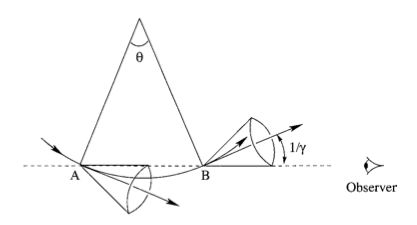
\includegraphics[width=0.75\textwidth]{chap0_intro/synchrotrondiagram.png}
    \caption[Diagram of electron gyration around a magnetic field line, resulting in synchrotron radiation.]{An electron gyrating around a magnetic field line, resulting in synchrotron radiation, from \citet{choudhuri2010astrophysics}.}
    \label{fig:synchrotrondiagram}
\end{figure}

Consider the time difference between radiation emitted at A and B. 

\begin{equation}
\Delta t=t_A-t_B=\frac{d}{c}-\left(\frac{\theta}{\omega}+\frac{d-R\theta}{c}\right)
\end{equation}
with $\theta\sim2/\gamma$ and $R=\omega v$. 

\begin{equation}
\Delta t = \frac{2m\gamma}{\gamma e B}-\frac{2mv\gamma}{\gamma eB c}=\frac{2m}{eB}(1-\beta)
\end{equation}
In the ultra-relativistic limit, $\beta\approx1-1/2\gamma^2$, giving $\Delta t=m/eB\gamma^2$. We thus expect the received radiation to have a strong frequency component at $f\sim1/\Delta t\to f\sim\gamma^2$. 

Then for charged particle motion in a uniform magnetic field, the Larmor formula for total power emitted picks up a factor of $\gamma^2$. Let the number of emitters with energy between $E$ and $E+dE$ be $E^{-p}dE$. Note that $E\propto\gamma$. These particles with energy $E$ radiate their power at $f\sim\gamma^2$ (see previous question), and there are $E^{-p}dE\sim f^{-p/2}df/f^{1/2}$, so the frequency spectrum is $f^{(-p+1)/2}df$. Many astrophysical particle distributions have $p\approx-2.5$, which gives $f(\nu)\propto\nu^{-0.75}$.
